\documentclass{article}

\usepackage{graphicx}
\usepackage{tikz}
\usepackage{tikzsymbols}
\usetikzlibrary{calc,patterns,shapes.geometric}
\pagestyle{empty}
\usepackage[margin=0pt]{geometry}
\geometry{papersize={14in,12in}}

\def\centerarc[#1](#2)(#3:#4:#5){\draw[#1] ($(#2)+({#5*cos(#3)},{#5*sin(#3)})$) arc (#3:#4:#5);}

\begin{document}
	\begin{figure}
		\centering
		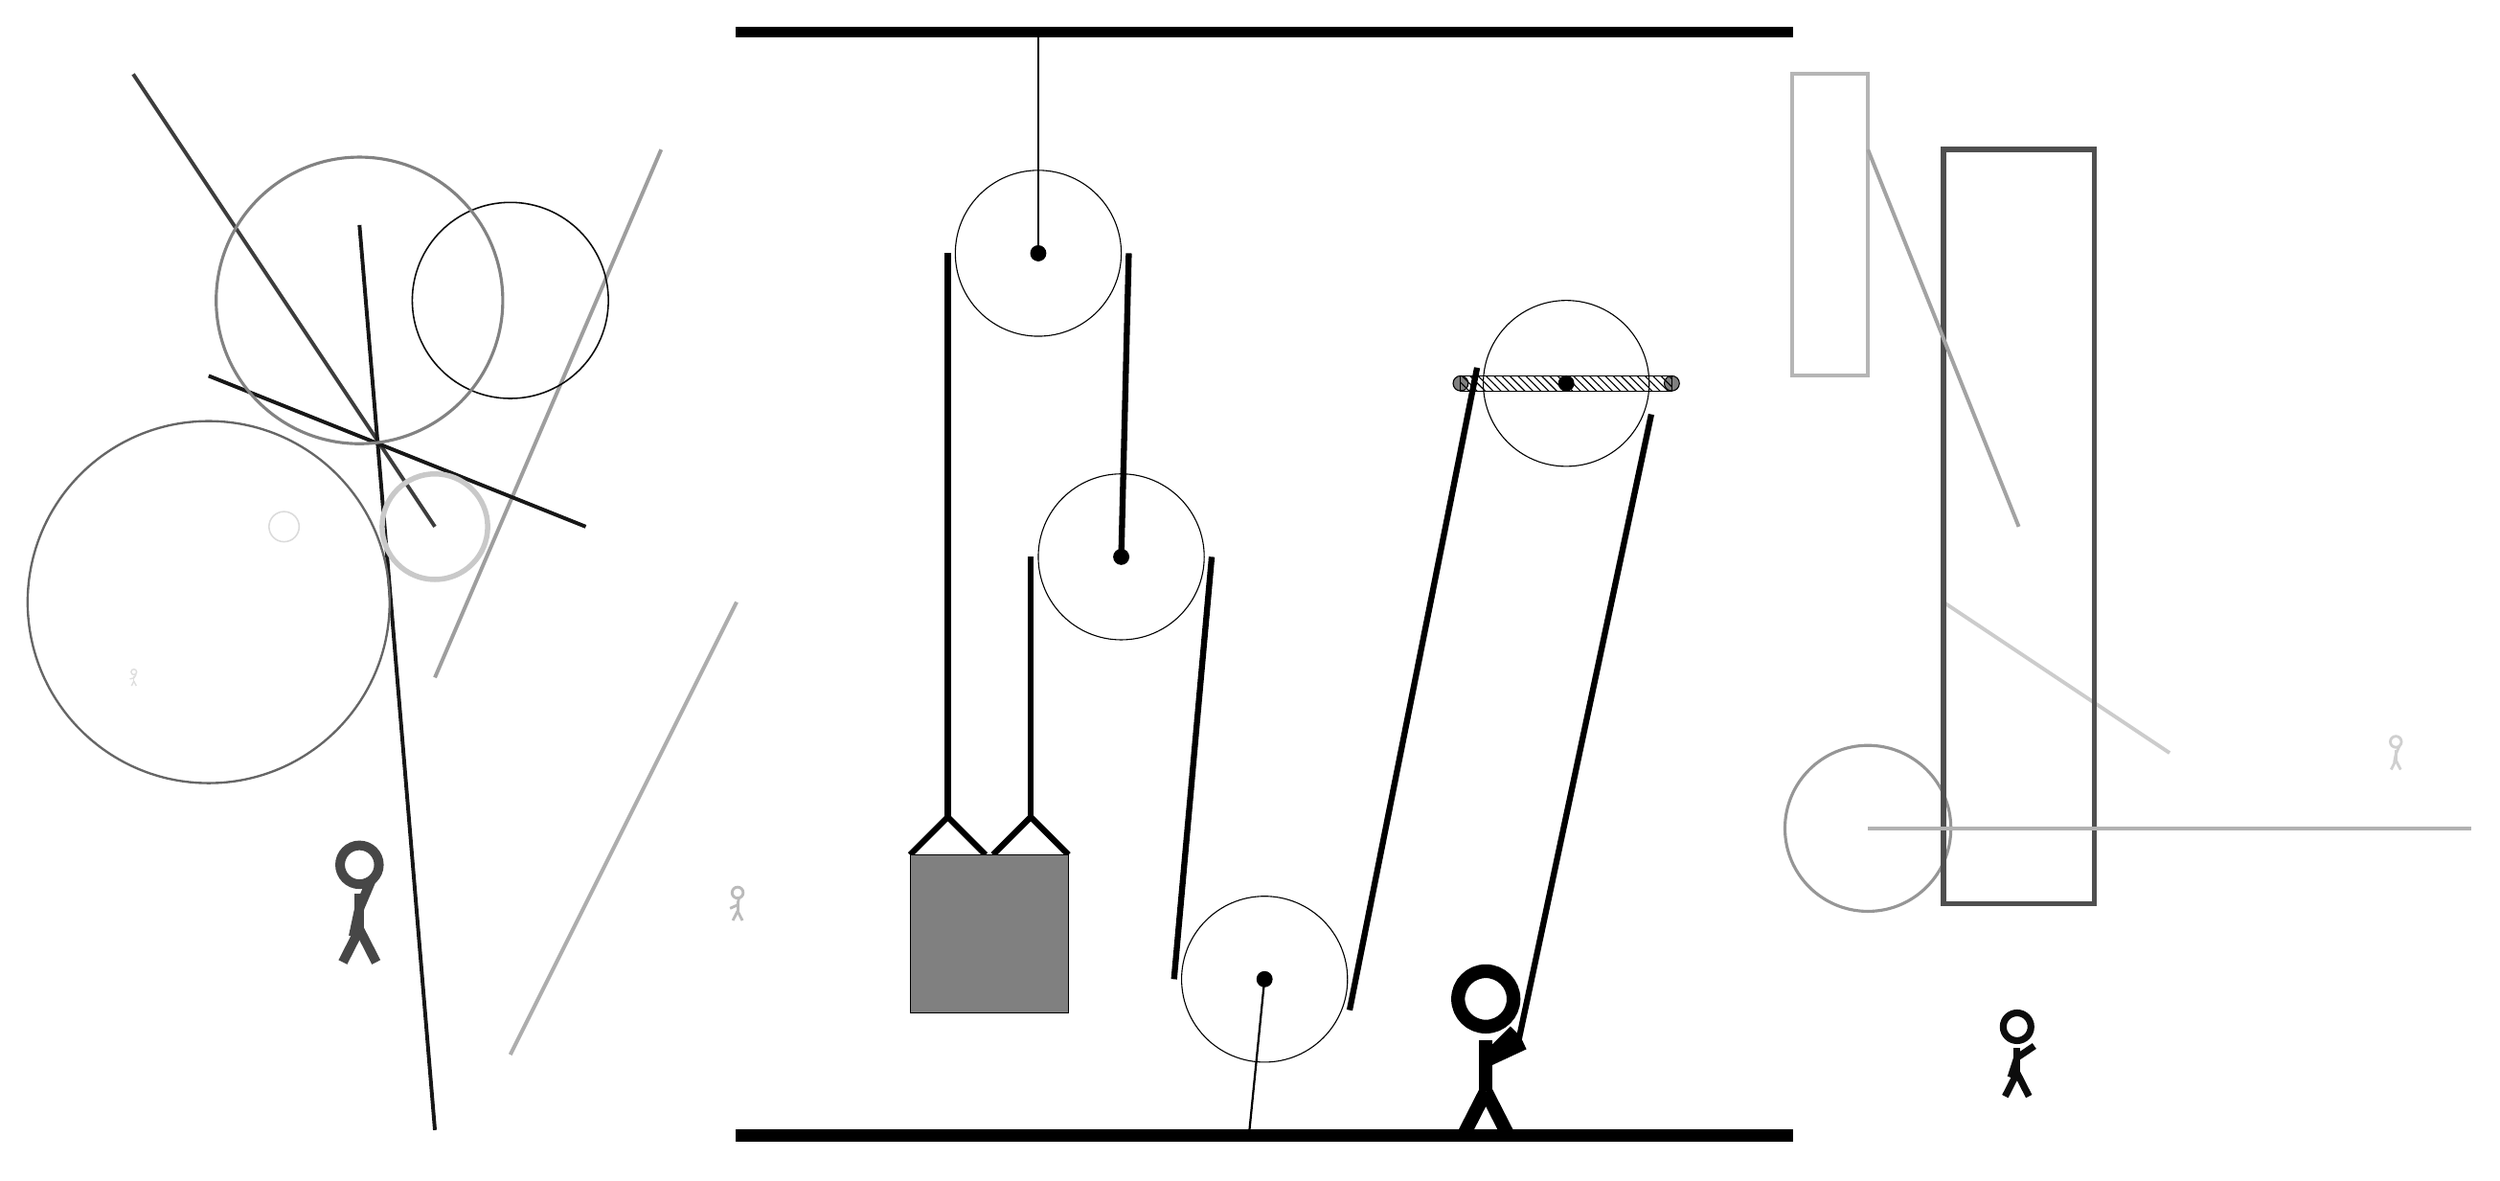
\begin{tikzpicture}
			%%%%% START %%%%%
			
			\draw[fill=black] (-2, 11.5) rectangle (12, 11.625);
			
			\draw (2, 8.625) circle (1.1);
			\draw[fill=black] (2, 8.625) circle (0.1);
			\draw[thick] (2, 8.625) -- (2, 11.5);
			
			\draw (3.1, 4.6) circle (1.1);
			\draw[fill=black] (3.1, 4.6) circle (0.1);
			
			\draw (5, -1) circle (1.1);
			\draw[fill=black] (5, -1) circle (0.1);
			\draw[thick] (5, -1) -- (4.8, -3);
			
			\draw (9, 6.9) circle (1.1);
			\draw[fill=black] (9, 6.9) circle (0.1);
			\draw[fill=black!50] (7.6, 6.9) circle (0.1);
			\draw[fill=black!50] (10.4, 6.9) circle (0.1);
			\draw[pattern=north west lines, pattern color=black] (7.6, 7.0) rectangle (10.4, 6.8);
			
			\draw[line width = 0.8mm]  (0.3, 0.65) -- (0.8, 1.15) -- (1.3, 0.65);
			\draw[line width = 0.8mm]  (1.4, 0.65) -- (1.9, 1.15) -- (2.4, 0.65);
			\draw[fill=black!50] (0.3, 0.65) rectangle (2.4, -1.45);
			
			\draw[line width = 0.8mm] (0.8, 8.625) -- (0.8, 1.15);
			\centerarc[line width = 0.8mm](2, 8.625)(0:180:1.2000000000000002);
			\draw[line width = 0.8mm] (3.2, 8.625) -- (3.1, 4.6);
			\draw[line width = 0.8mm] (1.9, 4.6) -- (1.9, 1.15);
			\centerarc[line width = 0.8mm](3.1, 4.6)(0:180:1.2000000000000002);
			\draw[line width = 0.8mm] (4.3, 4.6) -- (3.8, -1);
			\centerarc[line width = 0.8mm](5, -1)(180:340:1.2000000000000002);
			\draw[line width=0.8mm](6.1276, -1.4104) -- (7.8182, 7.1083);
			\centerarc[line width = 0.8mm](9, 6.9)(-20:170:1.2000000000000002);
			\draw[line width=0.8mm](10.1276, 6.4896) --  (8.35, -1.9);
			
			\node at (8, -2) {\Strichmaxerl[10][225][25]};
			
			\draw[line width=0.5mm, color=black!76](-6, 5) -- (-10, 11);
			
			\node[line width=0.5mm, color=black!95] at (15, -2) {\Strichmaxerl[5][72][34]};
			\node[line width=0.4mm, color=black!72] at (-7, 0) {\Strichmaxerl[7][78][67]};
			\draw [line width=0.4mm, color=black!41](13, 1) circle (1.1);
			\draw [line width=0.2mm, color=black!14](-8, 5) circle (0.2);
			
			\draw[line width=0.5mm, color=black!32](-2, 4) -- (-5, -2);
			\draw[line width=0.5mm, color=black!38](-3, 10) -- (-6, 3);
			\draw[line width=0.5mm, color=black!20](14, 4) -- (17, 2);
			\node[line width=0.7mm, color=black!19] at (20, 2) {\Strichmaxerl[2][79][67]};
			\draw[line width=0.5mm, color=black!91](-6, -3) -- (-7, 9);
			
			\draw[line width=0.5mm, color=black!91](-4, 5) -- (-9, 7);
			\draw[line width=0.5mm, color=black!29] (12, 11) rectangle (13, 7);
			\node[line width=0.2mm, color=black!13] at (-10, 3) {\Strichmaxerl[1][11][58]};
			
			\draw[line width=0.7mm, color=black!69] (14, 10) rectangle (16, 0);
			\draw [line width=0.7mm, color=black!21](-6, 5) circle (0.7);
			\draw [line width=0.2mm, color=black!96](-5, 8) circle (1.3);
			\node[line width=0.4mm, color=black!27] at (-2, 0) {\Strichmaxerl[2][24][80]};
			\draw [line width=0.4mm, color=black!49](-7, 8) circle (1.9);
			\draw[line width=0.5mm, color=black!36](13, 10) -- (15, 5);
			\draw [line width=0.3mm, color=black!60](-9, 4) circle (2.4);
			\draw[line width=0.5mm, color=black!30](13, 1) -- (21, 1);
			
			
			\draw[fill=black] (-2, -3) rectangle (12, -3.15);
			
			%%%%% END %%%%%
		\end{tikzpicture}
	\end{figure}	
\end{document}